\chapter{Blockchain-Grundlagen}
\label{cha:grundlagen}

\section{Funktionsweise}
Die Funktionsweise der Blockchain wird hauptsächlich an Bitcoin erklärt. Als erste Blockchain-Anwendung \cite{ZhengBlockchainChallengesOpportunities2017} und aufgrund der relativ geringen Komplexität liefert es die Grundlage für die Funktion der Technologie. Andere Implementationen, wie Ethereum oder Ripple, funktionieren nach dem gleichen Prinzip.

\subsection{Allgemein}
Wenn der Begriff ``Die Blockchain'' auftaucht, ist damit meistens die Blockchain-Technologie gemeint. Es gibt nicht nur eine global bestehende Blockchain und auch nicht nur eine Implementation der Technologie, was man an Bitcoin oder Ethereum sehen kann.

Allgemein kann man die Blockchain als Datenstruktur bezeichnen, welche verteilt, nicht löschbar und unmanipulierbar gespeichert werden kann. Weiterhin verifizieren jegliche Teilnehmer am Netzwerk ausgeführte Transaktionen, womit ein gemeinsamer Konsens über den Datenbestand besteht \cite{CrosbyBlockChainTechnologyBitcoin2016}.

%TODO: Speichert Fabric/Composer den Stand aller Daten ? Oder ergibt sich dieser aus den Transaktionen ?
%TODO: Klarmachen das Daten in der Blockchain geändert werden können. Die alten Daten sind aber trotzdem noch einsehbar, da die Transaktion dazu in der Blockchain besteht
%TODO: Metadaten Beispiele nennen ?
In einer Blockchain werden Transaktionen in Blöcken gespeichert. Dabei handelt es sich um Operationen, welche Daten erstellen, verändern, oder löschen. Aus diesen lässt sich letztendlich der aktuelle Datenbestand ermitteln. So erfolgt z.B. bei Bitcoin keine Speicherung des aktuellen Guthabens der Teilnehmer. Es wird nur aus allen bestehenden Transaktionen berechnet \cite{AntonopoulosMasteringbitcoin2015}. Die Daten welche letztendlich bestehen, können z.B. Geldtransferinformationen (Bitcoin), Smart Contracts (Ethereum, selbstausführende Verträge mit Programmlogik, siehe \ref{subsec:use-cases}), oder simple Dokumente oder Informationen sein \cite{EthereumWhitepaper2017}\cite{NakamotoBitcoinPeertoPeerElectronic2008}\cite{HyperledgerFabricTeamHyperledgerWhitepaper2016}. Die Blöcke setzen sich zusammen aus den Transaktionen sowie den Block Header, welcher verschiedene Metadaten, wie zum Beispiel den kombinierten Hash\footnote{Hash: Ergebnis einer Operation, welche ``eine Zeichenfolge beliebiger Länge auf eine Zeichenfolge mit fester Länge abbildet'' \cite{KryptologischeHashfunktion2017}.} aller Transaktionen, enthält \cite{AntonopoulosMasteringbitcoin2015}.

%TODO: Vielleicht lieber oberflächlicher bleiben ? Keine Unterscheidung zwischen Block und Block Header ?
Die Blöcke sind miteinander verkettet. Jeder Block Header enthält den Hash  des vorherigen Block Headers (Siehe Abb. \ref{fig:block-chain}). Dies ist ein wichtiges Feature zum Schutz der Blockchain vor Angriffen. Wenn ein Angreifer die Transaktionen eines Blocks zu seinen Gunsten verändern würde, würde sich der Hash des Block Headers ändern. Dieser müsste dann im darauffolgenden Block Header stehen, womit sich allerdings auch der Hash dieses Blocks ändert. Letztendlich müssten alle folgenden Blöcke manipuliert werden, um eine gültige Blockchain zu erhalten \cite{NakamotoBitcoinPeertoPeerElectronic2008}. Diese Manipulation wird durch verschiedene Verfahren erschwert, welche genauer in den Kapiteln \ref{subsec:konsens} und \ref{subsec:immutability} erklärt werden.

\begin{figure}[htb]
  \centering
	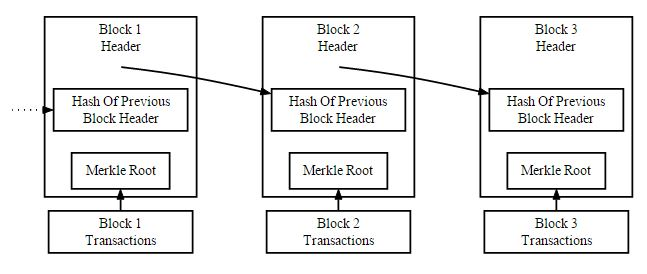
\includegraphics[width=0.85\textwidth,angle=0]{images/block-chain}
 	\caption{Verkettung von Blöcken durch Block Header Hashes}
	\label{fig:block-chain}
\end{figure}

Die Blockchain ist verteilt gespeichert. Jeder Teilnehmer hat die Möglichkeit Sie auf seinen Rechner zu speichern. Somit besteht keine zentrale Instanz, welche die Kontrolle über die Daten hat. Weiterhin gibt es keinen Single Point of Failure\footnote{Single Point of Failure: Komponente eines Systems, dessen Ausfall den Ausfall des gesamten Systems bewirkt \cite{SinglePointFailure2016}.},  \cite{CrosbyBlockChainTechnologyBitcoin2016}.

\label{subsec:konsens}
\subsection{Konsensmechanismen}
Aufgrund der verteilten Datenhaltung, muss es Verfahren geben, um die Daten synchron, und auf einen Stand, auf welchen sich alle Teilnehmer geeinigt haben, zu halten. Dazu gibt es die sogenannten Konsensmechanismen, welche gleichzeitig die Unmanipulierbarkeit der Daten sicherstellen. Bevor diese erklärt werden können, muss zunächst genauer auf die Funktion des Netzwerks eingegangen werden.

%TODO: Wann Validity-Check der Transaktionen ?
Wenn ein Teilnehmer eine Transaktion ausführt, wird diese, vorausgesetzt dass sie valide ist (Genauer im nächsten Absatz erklärt), an alle Nodes (Teilnehmer, welche die Blockchain speichern) im Netzwerk weitergeleitet. Diese werden in einen neuen Block aufgenommen, und jede Node beginnt mit der Erstellung von diesem. Das Erstellen wird durch verschiedene Konsensmechaniken realisiert. Bei Bitcoin und Ethereum findet der Proof-of-Work Anwendung (Genauer im folgenden Absatz erklärt). Sobald eine Node einen Block erstellt, wird dieser im Netzwerk verteilt. Jede Node hängt ihn an ihre lokale Blockchain an, und beginnt mit der Erstellung des nächsten Blocks \cite{NakamotoBitcoinPeertoPeerElectronic2008}\cite{EthereumWhitepaper2017}.

%TODO: Private und Public Key Footnode ?
Damit eine Transaktion valide ist, muss sie bestimmte Voraussetzungen erfüllen. So muss sie unter anderen mit den Private Key des Senders signiert sein. Mittels seines Public Keys kann überprüft werden, ob wirklich er der Sender der Nachricht ist und ob die Transaktion manipuliert wurde. Dies trägt zur Sicherheit der Blockchain bei, da ein Angreifer somit keine Transaktionen manipulieren oder im Namen eines anderen ausführen kann. In Bitcoin ist eine weitere Kondition, dass der Transaktionsersteller die zu sendenen Bitcoins besitzt \cite{AntonopoulosMasteringbitcoin2015}. In Systemen wie Ethereum und Hyperledger Fabric, in welchen eigene Programmlogik abgebildet werden kann, können Konditionen festgelegt werden. So muss z.B. ein Teilnehmer die nötigen Rechte haben um eine Transaktion auszuführen \cite{AccessControlLanguage}.

%TODO: Zeiten für die Erstellung erwähnen ? Wenn ja, auch Ethereum Zeit erwähnen
Der Proof-of-Work ist nur einer der zur Verfügung stehenden Konsensmechanismen. Er bedarf jedoch genauerer Erklärung, da er in den zwei bekanntesten Blockchain-Anwendungen (Bitcoin und Ethereum) erfolgreich genutzt wird, und  am meisten Erfolg verspricht (?)(Siehe Kapitel \ref{subsec:eval-konsens}). Der Proof-of-Work ist eine Art Rätsel, welches mit Rechenleistung gelöst werden muss, um einen Block zu erschaffen. Genauer gesagt, muss für einen Block ein Hash gefunden werden, welcher einen bestimmten Wert unterschreitet. Desto kleiner dieser ist, desto höher ist die Schwierigkeit. Um wachsender Rechenleistung und Teilnehmerzahl entgegen zu wirken, also die Zeit für die Erstellung eines Blockes ungefähr gleich zu halten, kann die Schwierigkeit angepasst werden. Dies ist aufgrund verschiedener Faktoren nötig, welche genauer im Kapitel \ref{sec:bc-problems} erläutert werden. Um unterschiedliche Hashwerte für gleiche Blöcke zu erhalten, gibt es im Block Header eine Nonce\footnote{Nonce: Eine ``Zahlen- oder Buchstabenkombination, [...] die nur ein einziges Mal in dem jeweiligen Kontext verwendet wird''\cite{Nonce2017}.}, welche verändert wird \cite{NakamotoBitcoinPeertoPeerElectronic2008}. Alle Nodes im Bitcoin-Netzwerk benötigen im Durchschnitt 10 Minuten um einen Proof-of-Work zu erbringen \cite{AntonopoulosMasteringbitcoin2015}, bei einer Hash Rate\footnote{Hash Rate: Anzahl der in einer Zeiteinheit berechneten Hashwerte \cite{GlossarBitcoin}.} von ca. 13.000.000 Terrahashes pro Sekunde \cite{HashRate}. Bei Ethereum beträgt die Zeit ungefähr 14 Sekunden \cite{EthereumAverageBlockTime}, bei einer Hash Rate von ca. 150 TH/s \cite{EthereumNetworkHashRate}.

Um vollständig zu verstehen, wie der Proof-of-Work funktioniert, muss das Forking erklärt werden. Wenn eine Node einen Proof-of-Work erbringt, also einen Block erstellt, wird dieser an alle anderen Nodes weitergeleitet. Im Bitcoin-Netzwerk dauert es bei einer maximalen Blockgröße von 1MB \cite{AntonopoulosMasteringbitcoin2015}, zwischen 6 und 20 Sekunden (Daten von 2017), bis ein Block mindestens 90\% aller Nodes erreicht hat \cite{BitcoinStatsb}. In dieser Zeit kann es vorkommen, dass eine weitere Node einen Block erstellt, bevor Sie den neuen Block erhält. Auch dieser wird im Netzwerk verteilt, womit 2 Versionen der Blockchain existieren: Eine endet mit Block A, und die andere mit Block B. Das Netzwerk muss sich nun darauf einigen, welche der beiden Versionen gültig ist. 



%TODO: Nodes = Teilnehmer, welche die Blockchain speichern.


\begin{itemize}
  \item Funktion (Wozu Konsensmechanismen ?) ==> Funktion des Netzwerks und Validität von Transaktionen
  \item Beispiel: Proof-of-Work
  \item Forking
\end{itemize}

\label{subsec:immutability}
\subsection{Angreifbarkeit/Immutability}
\begin{itemize}
  \item Wie sicher ist die Blockchain ?
\end{itemize}

\subsection{Blockchaintypen}
\begin{itemize}
  \item Public/Permissioned/Private Blockchains
\end{itemize}

\label{subsec:use-cases}
\section{Exemplarische Anwendungsfälle}
\begin{itemize}
    \item Wozu kann die Blockchain genutzt werden ?
\end{itemize}

\label{sec:bc-problems}
\section{Probleme für den B2B-Bereich}
\begin{itemize}
    \item Welche Nachteile hat die Blockchain im B2B-Bereich ?
    \item Blockerstellungszeit --> Warum konstant, 10 Minuten etc. ?
\end{itemize}
